\section{情景二：全程固定$q(t) \equiv q_0$,只用$c(t)$控制}
本节考虑第二类单一控制机制：在整个流行过程中固定隔离率
$q(t)\equiv q_0$，仅在压制期内动态调节接触率 $c(t)$，使社区感染人数维持在医疗容量红线
$I(t)=\eta$。系统为
\begin{equation}
\begin{cases}
\dot{S}(t)
=
-\dfrac{c(t)\big[\beta+q_0(1-\beta)\big]}{N}S(t)I(t), \\[.8em]
\dot{I}(t)
=
\dfrac{\beta c(t)(1-q_0)}{N}S(t)I(t)-\gamma I(t).
\end{cases}
\label{eq:s2:dynamics}
\end{equation}

控制函数写为
\begin{equation}
c(t)=
\begin{cases}
c_0, & t<t_1,\\
c_c(t), & t_1\leq t<t_2,\\
c_0, & t\geq t_2,
\end{cases}
\qquad
q(t)\equiv q_0 .
\label{eq:s2:piecewise-control}
\end{equation}
其中 $c_0$ 和 $q_0$ 分别表示常规接触水平和常规隔离水平。

在控制前后的常规防控阶段，仍使用与情景一一致的记号
\begin{equation}
\beta_1^0
=
\frac{c_0[\beta+q_0(1-\beta)]}{N},
\qquad
\beta_2^0
=
\frac{\beta c_0(1-q_0)}{N},
\label{eq:s2:beta12-phase0}
\end{equation}
并记
\begin{equation}
a=\frac{\beta_2^0}{\beta_1^0}
=
\frac{\beta(1-q_0)}{\beta+q_0(1-\beta)},
\qquad
\rho_1=\frac{\gamma}{\beta_1^0}
=
\frac{\gamma N}{c_0[\beta+q_0(1-\beta)]}.
\end{equation}
常规防控下的临界易感人数为
\begin{equation}
S_c
=
\frac{\gamma}{\beta_2^0}
=
\frac{\gamma N}{\beta c_0(1-q_0)}.
\label{eq:s2:Sc}
\end{equation}

\subsection{干预启动点 $S^*$ 与时间 $t_1$}

在干预启动前，情景二与情景一具有相同的常规防控背景，即 $c(t)=c_0$ 且 $q(t)=q_0$。因此启动点 $S^*$ 和启动时间 $t_1$ 仍由统一的常规阶段首次积分决定。具体地，
\begin{equation}
I(S)
=
I_0-a(S-S_0)+\rho_1\ln\frac{S}{S_0}.
\label{eq:s2:I-of-S-baseline}
\end{equation}
启动点 $S^*$ 由 $I(S^*)=\eta$ 给出，即
\begin{equation}
\eta-I_0+a(S^*-S_0)-\rho_1\ln\frac{S^*}{S_0}=0.
\label{eq:s2:Sstar-equation}
\end{equation}
等价地，
\begin{equation}
S^*
=
-S_c W_{-1}\left(
-\frac{S_0}{S_c}
\exp\left[-\frac{aS_0+I_0-\eta}{\rho_1}\right]
\right).
\label{eq:s2:Sstar-lambert}
\end{equation}
其中选取 Lambert $W$ 函数的 $-1$ 分支，是因为首次触碰红线发生在感染人数上升阶段，此时 $S^*>S_c$。确定 $S^*$ 后，启动时间为
\begin{equation}
t_1
=
\int_{S^*}^{S_0}
\frac{1}{\beta_1^0 S I(S)}\,dS .
\label{eq:s2:t1}
\end{equation}

\subsection{维持医疗红线所需的接触率控制}

在压制期 $t\in[t_1,t_2]$ 内要求 $I(t)\equiv\eta$，因此需要满足 $\dot I(t)=0$。由式 \eqref{eq:s2:dynamics} 第二式可得
\begin{equation}
\frac{\beta c_c(t)(1-q_0)}{N}S(t)\eta-\gamma\eta=0.
\end{equation}
由于 $\eta>0$，维持医疗红线所需的状态反馈接触率为
\begin{equation}
c_c(S)
=
\frac{\gamma N}{\beta(1-q_0)S}.
\label{eq:s2:c-control}
\end{equation}
这说明在固定隔离率 $q_0$ 的条件下，接触率必须随易感人数 $S(t)$ 的下降而逐渐上升，才能持续保持有效增长率为零。

\subsection{控制期内 $S(t)$ 的线性演化与控制结束时间}

将式 \eqref{eq:s2:c-control} 代入 $\dot S$ 方程，并利用 $I(t)=\eta$，得到
\begin{align}
\dot S(t)
&=
-\frac{1}{N}
\frac{\gamma N}{\beta(1-q_0)S(t)}
\big[\beta+q_0(1-\beta)\big]S(t)\eta \nonumber\\
&=
-\frac{\gamma\eta[\beta+q_0(1-\beta)]}{\beta(1-q_0)}
\doteq -K_c,
\label{eq:s2:Sdot-phase2}
\end{align}
其中
\begin{equation}
K_c
=
\frac{\gamma\eta[\beta+q_0(1-\beta)]}{\beta(1-q_0)}>0.
\label{eq:s2:Kc}
\end{equation}
因此控制期内易感人数线性下降：
\begin{equation}
S(t)
=
S^*-K_c(t-t_1),
\qquad
t_1\leq t\leq t_2.
\label{eq:s2:S-linear}
\end{equation}

由于控制结束后系统恢复到常规防控水平 $(c_0,q_0)$，解除控制点取为
\begin{equation}
S(t_2)=S_c=\frac{\gamma N}{\beta c_0(1-q_0)}.
\end{equation}
于是控制持续时间为
\begin{equation}
\Delta t_c
=
t_2-t_1
=
\frac{S^*-S_c}{K_c}
=
\frac{\beta(1-q_0)(S^*-S_c)}
{\gamma\eta[\beta+q_0(1-\beta)]}.
\label{eq:s2:delta-t}
\end{equation}
从而
\begin{equation}
t_2
=
t_1+
\frac{\beta(1-q_0)(S^*-S_c)}
{\gamma\eta[\beta+q_0(1-\beta)]}.
\label{eq:s2:t2}
\end{equation}

\subsection{时间域控制轨迹 $c_c(t)$}

将式 \eqref{eq:s2:S-linear} 代入状态反馈律 \eqref{eq:s2:c-control}，得到控制期内的时间域开环接触率：
\begin{equation}
c_c(t)
=
\frac{\gamma N}
{\beta(1-q_0)\left[S^*-K_c(t-t_1)\right]},
\qquad
t_1\leq t<t_2.
\label{eq:s2:c-time}
\end{equation}
等价地，利用终端条件 $S(t_2)=S_c$，也可写为
\begin{equation}
c_c(t)
=
\frac{\gamma N}
{\beta(1-q_0)\left[S_c+K_c(t_2-t)\right]}.
\label{eq:s2:c-time-remaining}
\end{equation}
控制期两端满足
\begin{equation}
c_c(t_1)
=
\frac{\gamma N}{\beta(1-q_0)S^*},
\qquad
c_c(t_2^-)
=
\frac{\gamma N}{\beta(1-q_0)S_c}
=c_0.
\label{eq:s2:c-endpoints}
\end{equation}
并且
\begin{equation}
\frac{dc_c(t)}{dt}
=
\frac{\gamma N K_c}
{\beta(1-q_0)S^2(t)}>0.
\end{equation}
因此 $c_c(t)$ 在控制期内严格递增，并在终点处与后期常规接触水平 $c_0$ 连续衔接。

\subsection{$c_c(t)$ 与参数的关系分析}

为与情景一保持平行，本节只考察两个具有直接政策含义的参数：
\[
c_0,\qquad \eta .
\]
以下分析均固定 $\beta,\gamma,q_0,N,S_0,I_0$，并假设医疗红线能够被首次触碰，即
$I_0\leq\eta<I_{\max}^{B}$ 且 $S^*>S_c$。

首先考虑启动点 $S^*$。由式 \eqref{eq:s2:Sstar-equation} 定义
\begin{equation}
F(S^*;c_0,\eta)
\doteq
\eta-I_0+a(S^*-S_0)-\rho_1\ln\frac{S^*}{S_0}
=0.
\label{eq:s2:F-Sstar}
\end{equation}
由于
\begin{equation}
F_S
=
a-\frac{\rho_1}{S^*}
=
a\left(1-\frac{S_c}{S^*}\right)>0,
\end{equation}
隐函数定理给出
\begin{equation}
\frac{\partial S^*}{\partial\eta}
=
-\frac{1}{F_S}<0.
\label{eq:s2:Sstar-eta-sign}
\end{equation}
另一方面，$a$ 与 $c_0$ 无关，而
\[
\frac{\partial\rho_1}{\partial c_0}
=
-\frac{\rho_1}{c_0}.
\]
因此
\begin{equation}
F_{c_0}
=
\frac{\rho_1}{c_0}\ln\frac{S^*}{S_0}<0,
\end{equation}
从而
\begin{equation}
\frac{\partial S^*}{\partial c_0}
=
-\frac{F_{c_0}}{F_S}>0.
\label{eq:s2:Sstar-c0-sign}
\end{equation}
这与情景一相同：医疗容量阈值越高，触碰红线时易感人数越低；常规接触水平越高，系统越早触碰红线，触碰时易感人数越高。

接下来用相对接触削减强度刻画控制强度：
\begin{equation}
u_c(t)
=
1-\frac{c_c(t)}{c_0}.
\end{equation}
由 $c_c(S)/c_0=S_c/S$ 可得
\begin{equation}
u_c(S)
=
1-\frac{S_c}{S}.
\label{eq:s2:u-state}
\end{equation}
由于控制期内 $S(t)$ 从 $S^*$ 单调下降到 $S_c$，$u_c(t)$ 从最大值单调下降到 $0$，其中
\begin{equation}
u_{\max}
=
u_c(t_1)
=
1-\frac{S_c}{S^*}.
\label{eq:s2:umax}
\end{equation}
对 $\eta$ 而言，$S_c$ 不变而 $S^*_\eta<0$，因此
\begin{equation}
\frac{\partial u_{\max}}{\partial\eta}
=
\frac{S_c}{(S^*)^2}\frac{\partial S^*}{\partial\eta}<0.
\end{equation}
对 $c_0$ 而言，$S_{c,c_0}=-S_c/c_0$ 且 $S^*_{c_0}>0$，所以
\begin{equation}
\frac{\partial u_{\max}}{\partial c_0}
=
\frac{S_c}{c_0S^*}
+
\frac{S_c}{(S^*)^2}
\frac{\partial S^*}{\partial c_0}>0.
\end{equation}
因此，医疗容量越高，所需最大接触削减越小；常规接触水平越高，所需最大接触削减越大。

若采用启动后的相对时间 $\tau=t-t_1$，则
\begin{equation}
S(\tau)=S^*-K_c\tau,
\qquad
u_c(\tau)=1-\frac{S_c}{S^*-K_c\tau}.
\label{eq:s2:u-tau}
\end{equation}
在固定 $\tau$ 下，$K_c$ 与 $c_0$ 无关，但与 $\eta$ 成正比。于是
\begin{equation}
\frac{\partial S(\tau)}{\partial\eta}
=
\frac{\partial S^*}{\partial\eta}
-\frac{K_c}{\eta}\tau<0,
\end{equation}
从而 $\partial u_c(\tau)/\partial\eta<0$。而
\begin{equation}
\frac{\partial u_c(\tau)}{\partial c_0}
=
\frac{S_c}{c_0S(\tau)}
+
\frac{S_c}{S^2(\tau)}
\frac{\partial S^*}{\partial c_0}>0.
\end{equation}
因此，在相同已控制时间 $\tau$ 处，增大 $\eta$ 会降低所需接触削减强度，而增大 $c_0$ 会提高所需接触削减强度。

启动时间 $t_1$ 的分析与情景一相同。由
\begin{equation}
t_1
=
\frac{N}{c_0[\beta+q_0(1-\beta)]}
\int_{S^*}^{S_0}
\frac{1}{S I(S;c_0)}\,dS
\end{equation}
可得
\begin{equation}
\frac{\partial t_1}{\partial\eta}>0,
\qquad
\frac{\partial t_1}{\partial c_0}<0.
\end{equation}
即医疗容量越高，触碰红线越晚；常规接触水平越高，触碰红线越早。

控制持续时间为
\begin{equation}
\Delta t_c
=
\frac{S^*-S_c}{K_c}.
\end{equation}
由于 $K_c$ 与 $\eta$ 成正比，而 $S^*_\eta<0$、$S_c$ 不依赖 $\eta$，有
\begin{equation}
\frac{\partial\Delta t_c}{\partial\eta}
=
\frac{1}{K_c}\frac{\partial S^*}{\partial\eta}
-
\frac{S^*-S_c}{K_c\eta}<0.
\end{equation}
另一方面，$K_c$ 与 $c_0$ 无关，且
\begin{equation}
\frac{\partial(S^*-S_c)}{\partial c_0}
=
\frac{\partial S^*}{\partial c_0}+\frac{S_c}{c_0}>0,
\end{equation}
因此
\begin{equation}
\frac{\partial\Delta t_c}{\partial c_0}>0.
\end{equation}
最后，$t_2=t_1+\Delta t_c$。由于 $t_1$ 与 $\Delta t_c$ 对 $c_0$ 和 $\eta$ 的变化方向相反，$t_2$ 的整体单调性不宜在一般参数条件下强行判断，应结合数值结果讨论。

\subsection{数值分析}

本节数值示例与情景一保持相同参数：
\[
N=763,\qquad q_0=0.05,\qquad c_0=10,\qquad \gamma=0.1,
\]
并令
\[
R_0=\frac{\beta c_0(1-q_0)}{\gamma}=3.5,
\qquad
\eta=0.05N=38.15.
\]
数值程序 \texttt{scenario2\_c\_control\_fixed\_q0.m} 使用解析得到的时间域开环控制 $c_c(t)$，并将系统分为 $[0,t_1]$、$[t_1,t_2]$ 和 $[t_2,T]$ 三段积分。图~\ref{fig:scenario2_single_sim} 显示，受控情形下 $I(t)$ 在控制期内贴近医疗红线 $\eta$，且 $c_c(t)$ 从较低水平逐渐上升并在 $t_2$ 处回到 $c_0$，验证了上述解析推导。

\begin{figure}[h]
    \centering
    \caption{情景二中固定隔离率、动态接触率控制的时间演化}
    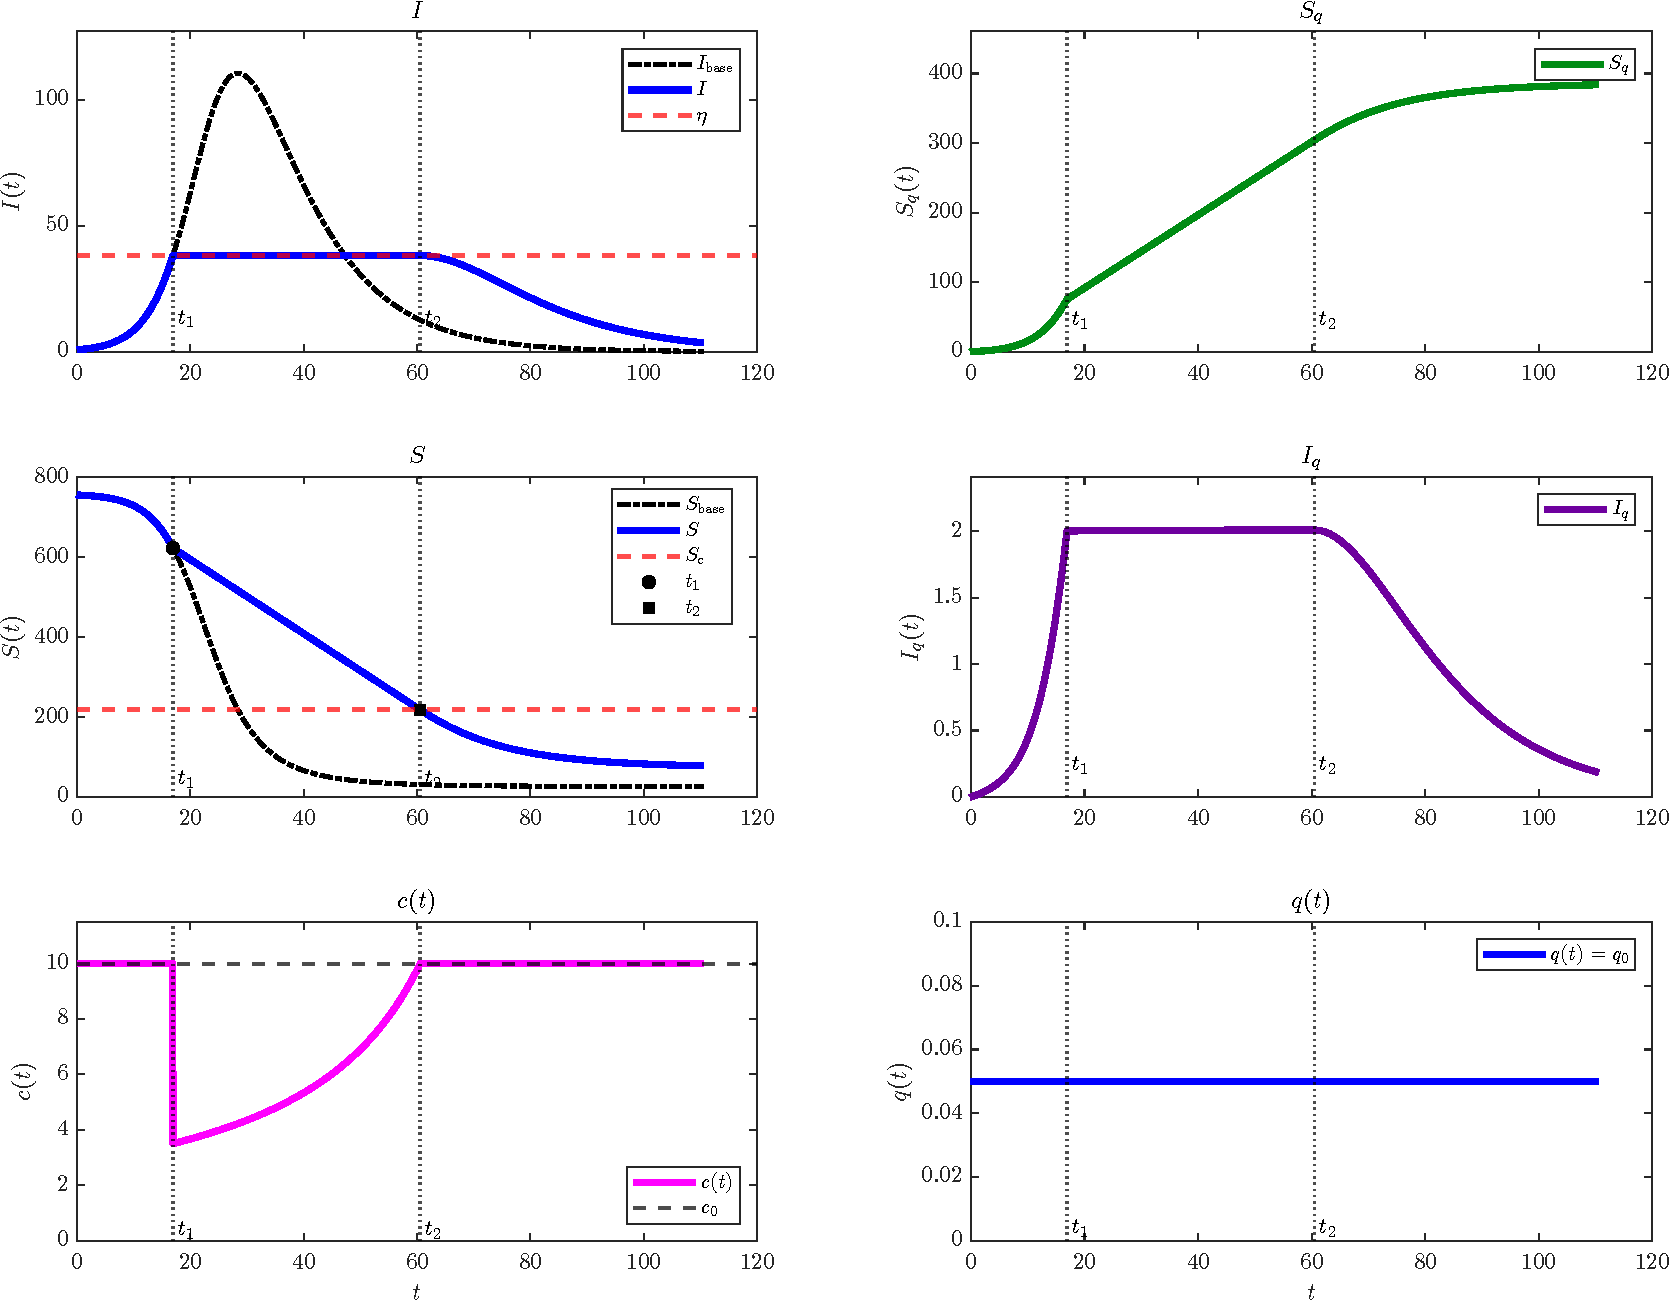
\includegraphics[width=0.7\textwidth]{figures/scenario2_c_control_fixed_q0.pdf}
    \label{fig:scenario2_single_sim}
\end{figure}

为了进一步考察参数影响，我们编写数值程序 \texttt{scenario2\_parameter\_analysis.m}。与理论分析一致，该程序只考察两个参数 $c_0$ 与 $\eta$：第一组数值实验固定 $\beta,\gamma,q_0,N,S_0,I_0,\eta$，改变常规接触水平 $c_0$；第二组数值实验固定 $\beta,\gamma,c_0,q_0,N,S_0,I_0$，改变医疗容量阈值 $\eta$。

对每组参数，程序首先判断常规防控背景下是否能够触及 $I=\eta$。若可行，则计算 $S^*$、$S_c$、$t_1$、$t_2$、控制持续时间 $\Delta t_c$、最大接触削减强度
\[
u_{\max}=1-\frac{c_c(t_1)}{c_0}=1-\frac{S_c}{S^*},
\]
以及累计接触削减强度
\begin{equation}
J_c
=
\int_{t_1}^{t_2}\left(1-\frac{c_c(t)}{c_0}\right)\,dt.
\end{equation}

\begin{table}[htbp]
  \centering
  \footnotesize
  \caption{情景二中不同 $c_0$ 下的关键控制指标。}
  \label{tab:scenario2_c0_summary}
  \begin{tabular}{ccccccc}
\toprule
$c_0$ & $S^*$ & $S_c$ & $t_1$ & $\Delta t$ & $u_{\max}$ & $J_c$ \\
\midrule
6 & 547.9037 & 363.3333 & 42.0849 & 19.9212 & 0.3369 & 3.8123 \\
7 & 584.9426 & 311.4286 & 30.4242 & 29.5212 & 0.4676 & 8.3332 \\
8 & 603.3308 & 272.5000 & 23.9821 & 35.7076 & 0.5483 & 12.3303 \\
9 & 614.6298 & 242.2222 & 19.8289 & 40.1951 & 0.6059 & 15.8509 \\
10 & 622.3428 & 218.0000 & 16.9150 & 43.6420 & 0.6497 & 18.9597 \\
11 & 627.9638 & 198.1818 & 14.7533 & 46.3877 & 0.6844 & 21.7182 \\
12 & 632.2505 & 181.6667 & 13.0843 & 48.6329 & 0.7127 & 24.1797 \\
13 & 635.6311 & 167.6923 & 11.7560 & 50.5061 & 0.7362 & 26.3887 \\
\bottomrule
\end{tabular}

\end{table}

\begin{table}[htbp]
  \centering
  \footnotesize
  \caption{情景二中不同 $\eta$ 下的关键控制指标。}
  \label{tab:scenario2_eta_summary}
  \begin{tabular}{cccccccc}
\toprule
$\eta$ & $\eta/N$ & $S^*$ & $S_c$ & $t_1$ & $\Delta t$ & $u_{\max}$ & $J_c$ \\
\midrule
15.2600 & 0.020 & 705.1720 & 218.0000 & 12.4872 & 131.4549 & 0.6909 & 62.3993 \\
19.0750 & 0.025 & 691.7028 & 218.0000 & 13.4993 & 102.2564 & 0.6848 & 47.9194 \\
22.8900 & 0.030 & 678.1118 & 218.0000 & 14.3502 & 82.7688 & 0.6785 & 38.2662 \\
26.7050 & 0.035 & 664.3904 & 218.0000 & 15.0914 & 68.8290 & 0.6719 & 31.3710 \\
30.5200 & 0.040 & 650.5291 & 218.0000 & 15.7536 & 58.3552 & 0.6649 & 26.1996 \\
34.3350 & 0.045 & 636.5172 & 218.0000 & 16.3568 & 50.1909 & 0.6575 & 22.1774 \\
38.1500 & 0.050 & 622.3428 & 218.0000 & 16.9150 & 43.6420 & 0.6497 & 18.9597 \\
\bottomrule
\end{tabular}

\end{table}

\begin{figure}[htbp]
    \centering
    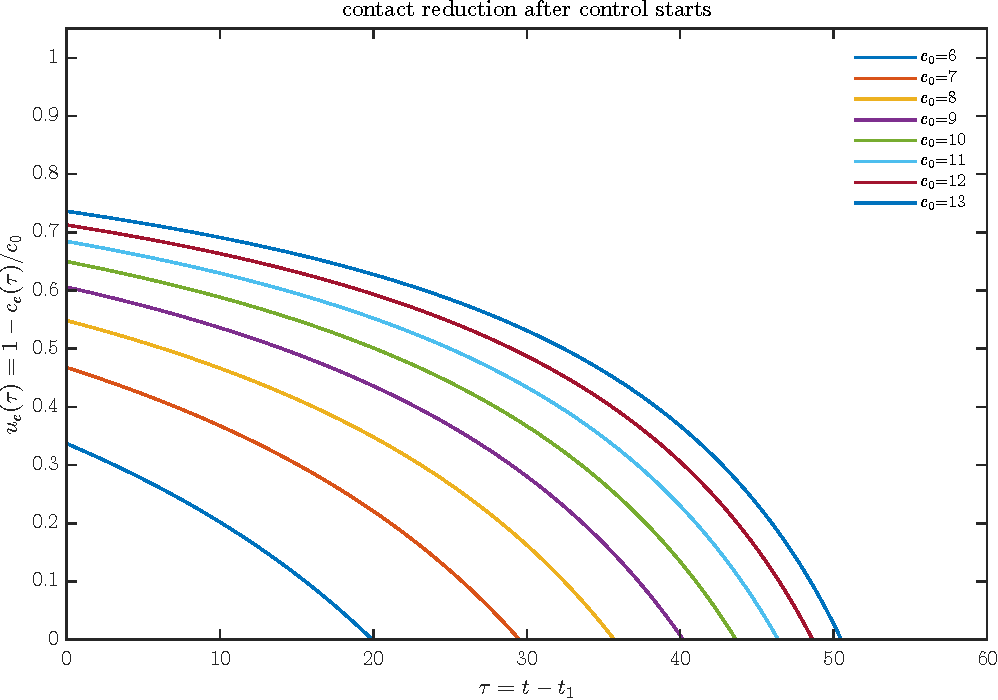
\includegraphics[width=0.72\textwidth]{figures/scenario2_u_tau_c0.pdf}
    \caption{情景二中不同 $c_0$ 下启动后相对时间中的接触削减强度 $u_c(\tau)$。}
    \label{fig:scenario2_u_tau_c0}
\end{figure}

\begin{figure}[htbp]
    \centering
    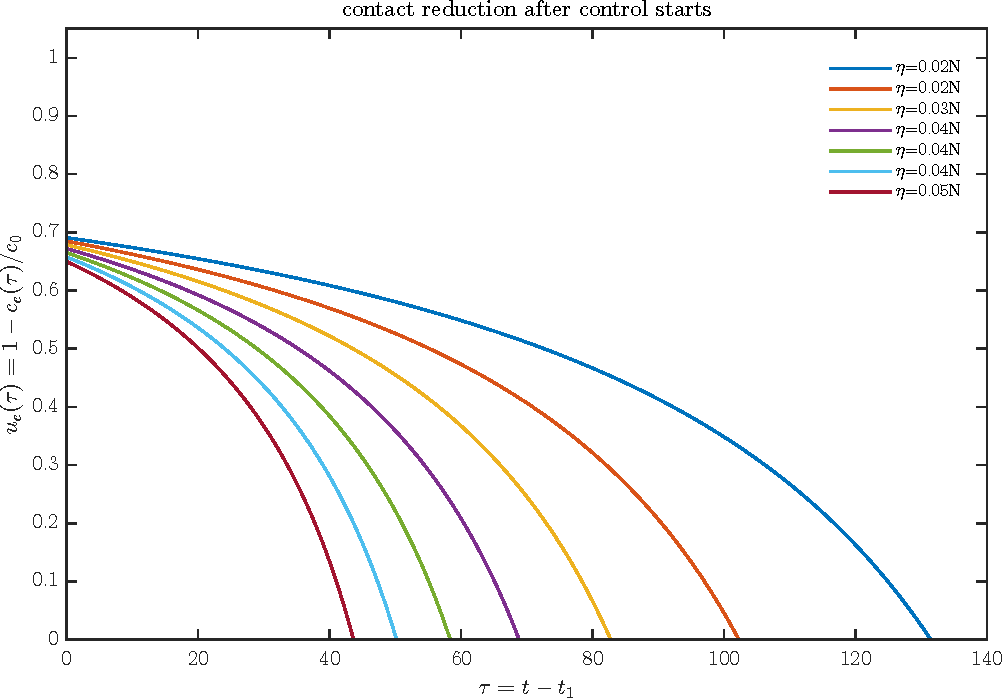
\includegraphics[width=0.72\textwidth]{figures/scenario2_u_tau_eta.pdf}
    \caption{情景二中不同 $\eta$ 下启动后相对时间中的接触削减强度 $u_c(\tau)$。}
    \label{fig:scenario2_u_tau_eta}
\end{figure}

\begin{figure}[htbp]
    \centering
    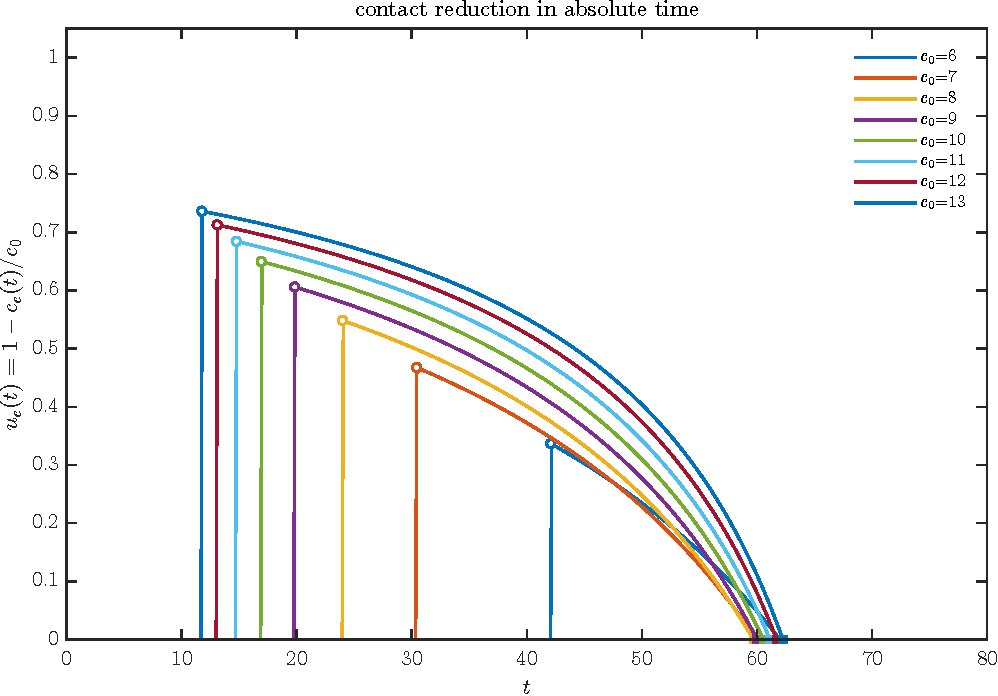
\includegraphics[width=0.72\textwidth]{figures/scenario2_u_time_c0.pdf}
    \caption{情景二中不同 $c_0$ 下绝对时间中的接触削减强度 $u_c(t)$。}
    \label{fig:scenario2_u_time_c0}
\end{figure}

\begin{figure}[htbp]
    \centering
    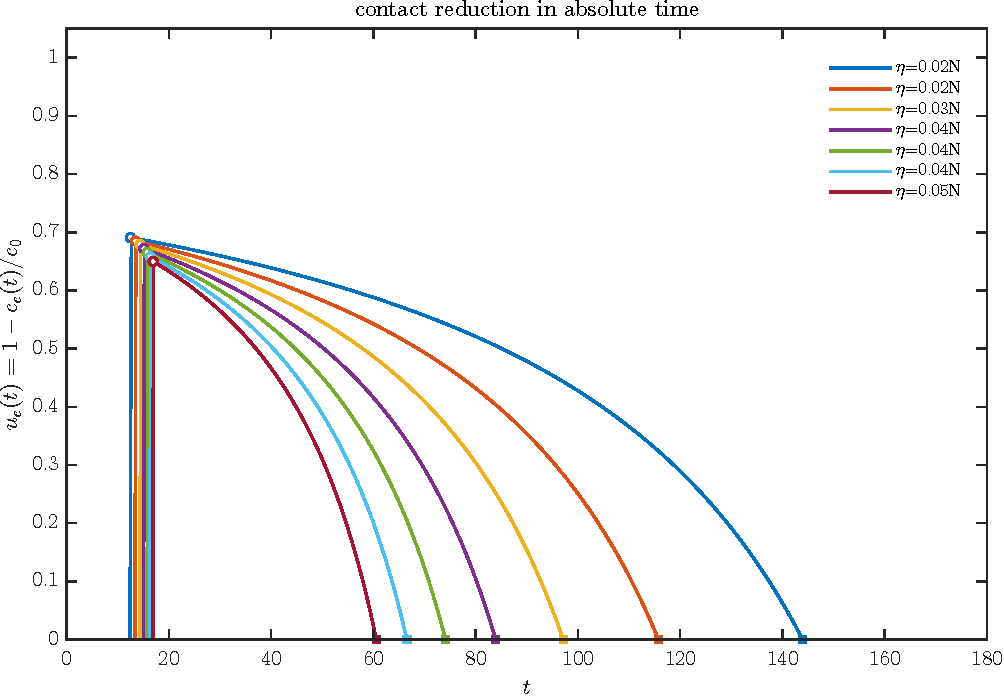
\includegraphics[width=0.72\textwidth]{figures/scenario2_u_time_eta.pdf}
    \caption{情景二中不同 $\eta$ 下绝对时间中的接触削减强度 $u_c(t)$。}
    \label{fig:scenario2_u_time_eta}
\end{figure}

\begin{figure}[htbp]
    \centering
    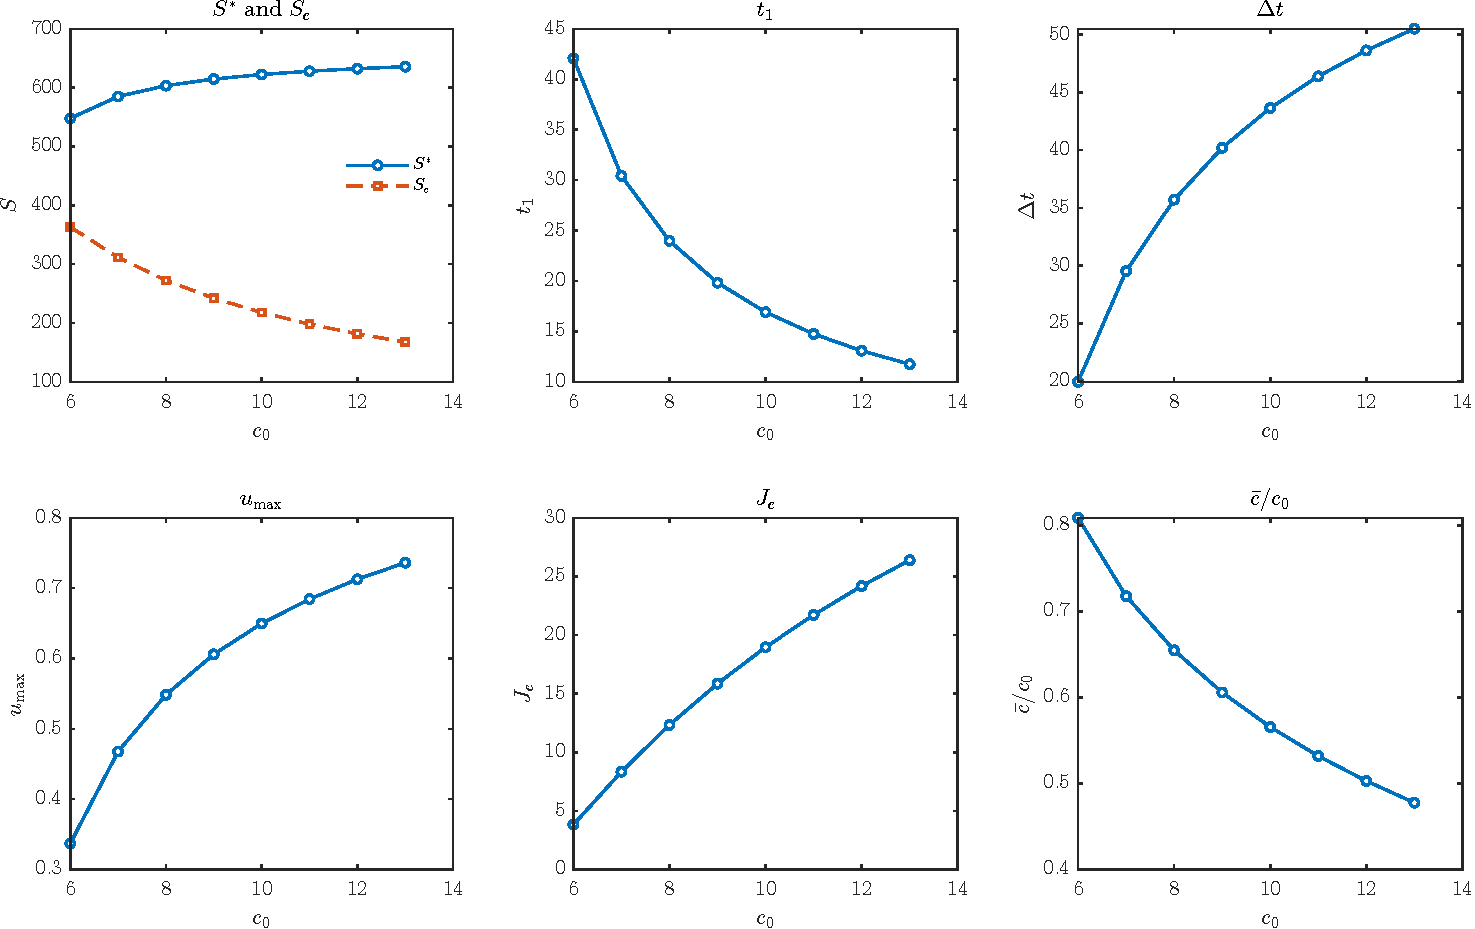
\includegraphics[width=0.88\textwidth]{figures/scenario2_summary_c0.pdf}
    \caption{情景二中关键指标随 $c_0$ 的变化。}
    \label{fig:scenario2_summary_c0}
\end{figure}

\begin{figure}[htbp]
    \centering
    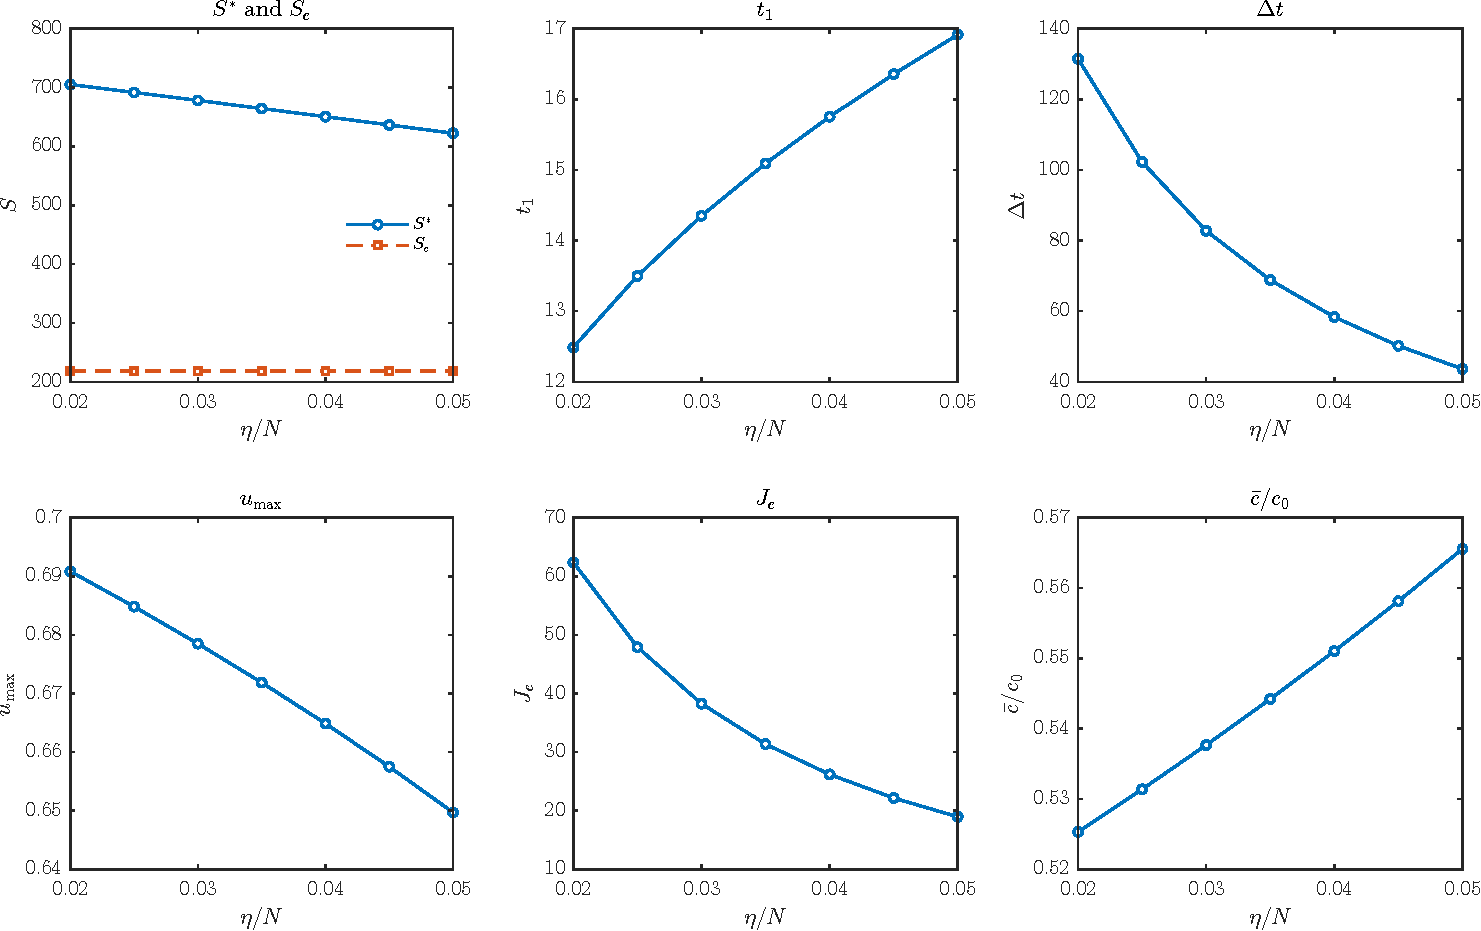
\includegraphics[width=0.88\textwidth]{figures/scenario2_summary_eta.pdf}
    \caption{情景二中关键指标随 $\eta$ 的变化。}
    \label{fig:scenario2_summary_eta}
\end{figure}

\begin{figure}[htbp]
    \centering
    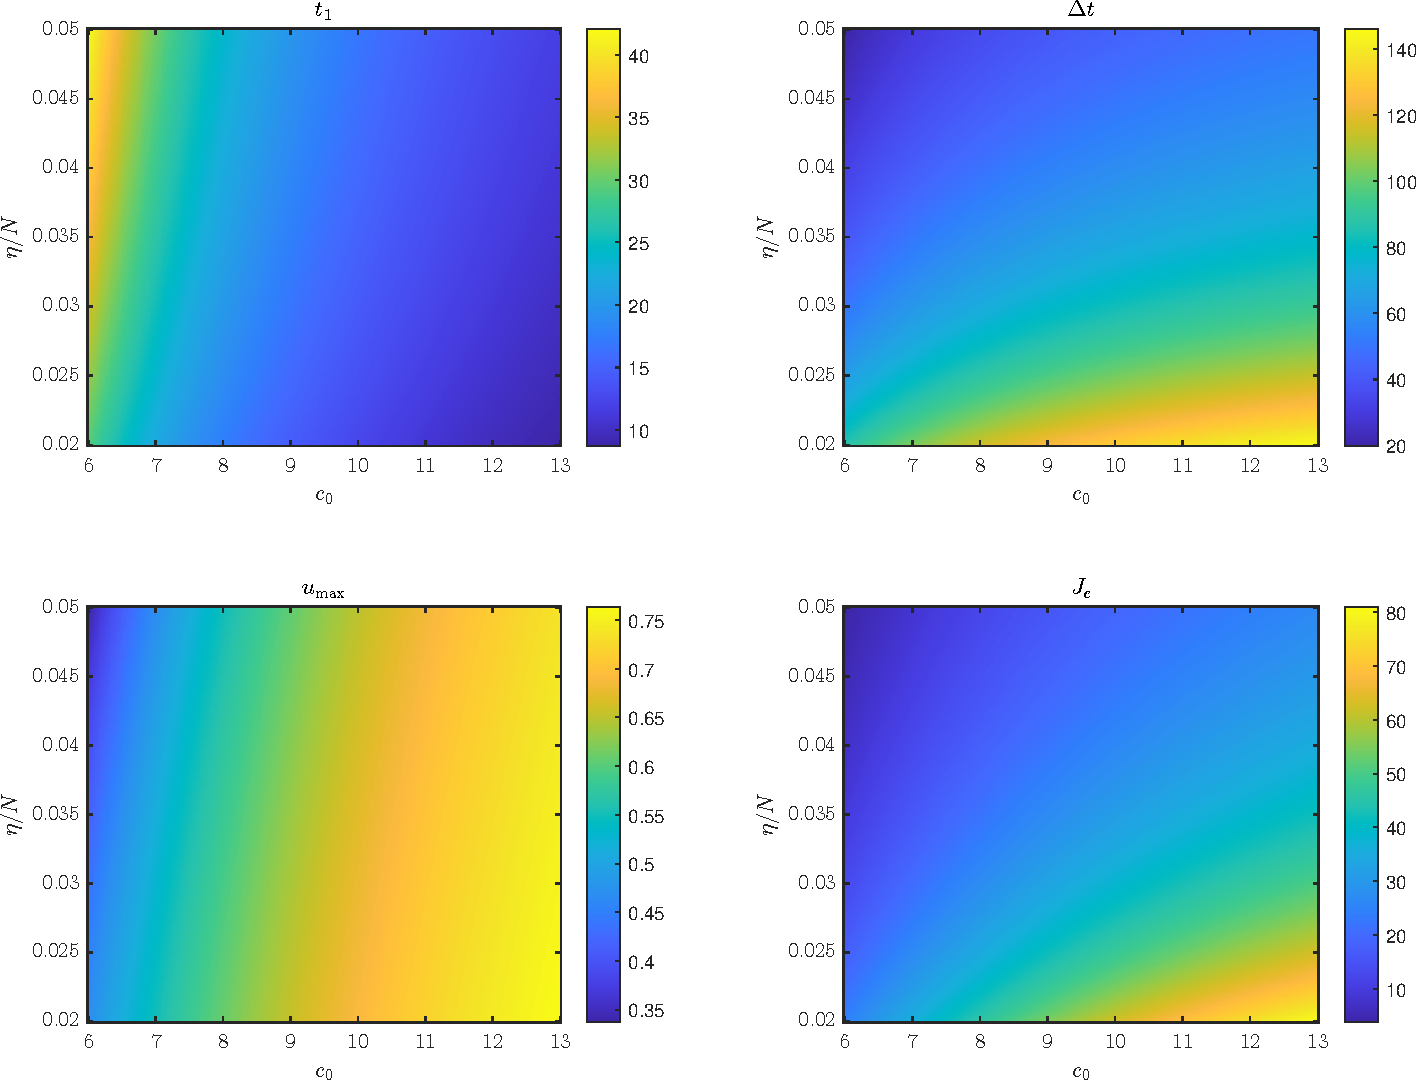
\includegraphics[width=0.88\textwidth]{figures/scenario2_heatmaps_c0_eta.pdf}
    \caption{情景二中 $(c_0,\eta)$ 平面上的 $t_1$、$\Delta t_c$、$u_{\max}$ 与 $J_c$ 热图。}
    \label{fig:scenario2_heatmaps_c0_eta}
\end{figure}

\begin{figure}[htbp]
    \centering
    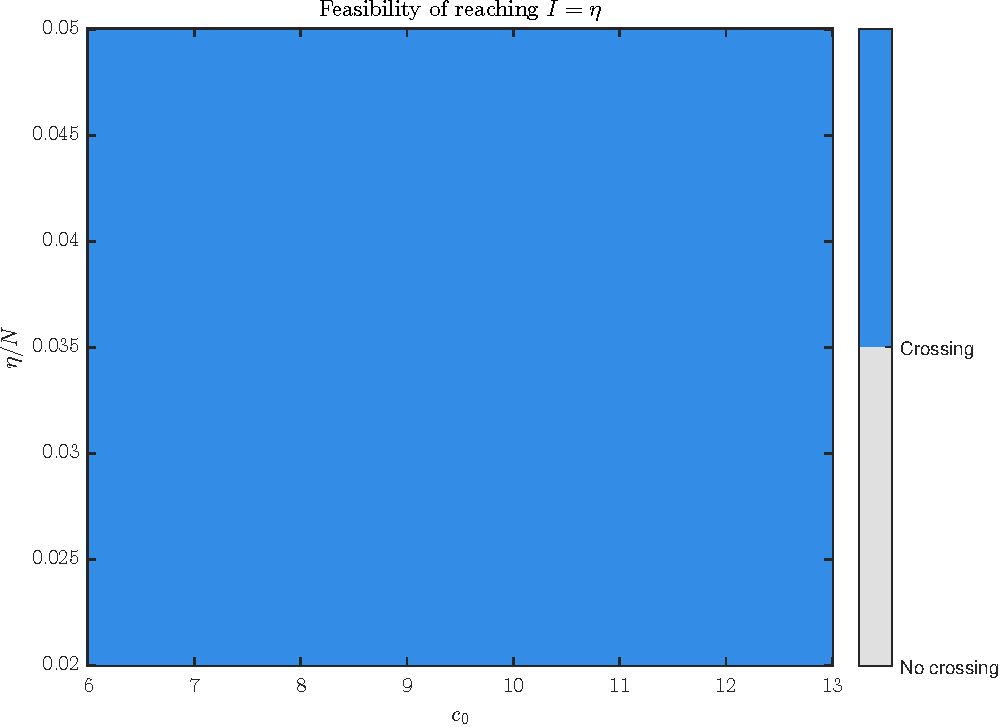
\includegraphics[width=0.68\textwidth]{figures/scenario2_feasibility_c0_eta.pdf}
    \caption{情景二中 $(c_0,\eta)$ 平面上是否能够触及 $I=\eta$ 的可行性区域。}
    \label{fig:scenario2_feasibility_c0_eta}
\end{figure}

从表~\ref{tab:scenario2_c0_summary} 和图~\ref{fig:scenario2_summary_c0} 可以看出，随着 $c_0$ 增大，系统更早触碰红线，$S^*$ 上升而 $S_c$ 下降，因此控制区间变长，所需最大接触削减强度 $u_{\max}$ 增大，累计控制强度 $J_c$ 也随之增大。这与理论分析中 $S^*_{c_0}>0$、$t_{1,c_0}<0$、$\Delta t_{c_0}>0$ 以及 $u_{\max,c_0}>0$ 的结论一致。

从表~\ref{tab:scenario2_eta_summary} 和图~\ref{fig:scenario2_summary_eta} 可以看出，随着医疗容量阈值 $\eta$ 增大，系统更晚触碰红线，$S^*$ 下降，控制持续时间、最大接触削减强度以及累计接触削减强度均下降。这与理论分析中 $S^*_\eta<0$、$t_{1,\eta}>0$、$\Delta t_\eta<0$ 以及 $u_{\max,\eta}<0$ 的结论一致。图~\ref{fig:scenario2_heatmaps_c0_eta} 和图~\ref{fig:scenario2_feasibility_c0_eta} 进一步展示了 $(c_0,\eta)$ 平面上的关键指标变化与可行性区域。

\section{情景三：同时调节$c(t)$和$q(t)$}

在前述解析推导中，我们或者假设 $c(t)\equiv c_0$，只用 $q(t)$ 控制；或者假设 $q(t)\equiv q_0$，只用 $c(t)$ 控制。实际上，在政策执行中，减少接触和提高追踪隔离往往可以同时进行。因此本节考虑如下联合控制策略：在疫情触及 ICU 医疗红线之前，系统采用背景水平
\begin{equation}
c(t)\equiv c_0,\qquad q(t)\equiv q_0,
\end{equation}
当 $I(t)$ 首次达到 $\eta$ 后，再按给定权重同时调节 $c(t)$ 与 $q(t)$，使得 $I(t)\equiv \eta$。

\subsection{干预启动点 $S^*$ 与时间 $t_1$}
在干预启动前 $c(t)=c_0$ 且 $q(t)=q_0$。因此启动点 $S^*$ 和启动时间 $t_1$ 仍由统一的常规阶段首次积分 \eqref{eq:model:first-integral} 决定。具体地，$S^*$ 满足
\begin{equation}
\frac{\beta_2^0}{\beta_1^0}S^*-\rho_1\ln S^*
=
C_0-\eta,
\label{eq:s3:Sstar-equation}
\end{equation}
因此
\begin{equation}
S^*
=
-S_c W_{-1}\left(
-\frac{1}{S_c}\exp\left[-\frac{C_0-\eta}{\rho_1}\right]
\right),
\label{eq:s3:Sstar-lambert}
\end{equation}
确定 $S^*$ 后，启动时间为
\begin{equation}
t_1
=
\int_{S_0}^{S^*}
\frac{1}{-\beta_1^0 S\left[
C_0-\frac{\beta_2^0}{\beta_1^0}S+\rho_1\ln S
\right]}\,dS.
\label{eq:s3:t1}
\end{equation}
该积分通常通过数值求积计算。


\subsection{权重下的联合控制律}

在控制期 $t\in[t_1,t_2]$，要求
\begin{equation}
I(t)\equiv \eta,\qquad \dot I(t)=0.
\end{equation}
由 $\dot I=0$ 得到维持医疗红线所需的联合控制方程
\begin{equation}
\beta c(t)(1-q(t))S(t)=\gamma.
\label{eq:s3:joint-control}
\end{equation}
此时加强防控阶段的系数为
\begin{equation}
\beta_1^1(t)=c(t)\big[\beta+q(t)(1-\beta)\big],
\qquad
\beta_2^1(t)=\beta c(t)(1-q(t)).
\label{eq:s3:beta12-phase1}
\end{equation}
式 \eqref{eq:s3:joint-control} 只给出了 $(c,q)$ 平面上的一条控制曲线，不能唯一确定 $c(t)$ 和 $q(t)$。因此需要进一步规定两种控制手段如何分担同一个总控制强度。

为此，先将两种控制强度归一化。定义
\begin{equation}
u_c(t)=1-\frac{c(t)}{c_0},
\qquad
u_q(t)=\frac{q(t)-q_0}{1-q_0}.
\label{eq:s3:normalized-controls}
\end{equation}
其中 $u_c(t)$ 表示接触率相对于背景水平 $c_0$ 的下降比例，$u_q(t)$ 表示隔离率在其可提升空间 $[q_0,1]$ 中已经使用的比例。进一步引入总控制强度 $u(t)$ 和控制分担权重 $\omega\in[0,1]$，并规定
\begin{equation}
u_c(t)=(1-\omega)u(t),
\qquad
u_q(t)=\omega u(t).
\label{eq:s3:strict-weight}
\end{equation}
于是
\begin{equation}
c(t)=c_0[1-(1-\omega)u(t)],
\qquad
q(t)=q_0+(1-q_0)\omega u(t).
\label{eq:s3:cq-u}
\end{equation}
这里 $\omega$ 是严格意义下的权重：$\omega=0$ 表示总控制强度完全由接触率控制承担；$\omega=1$ 表示总控制强度完全由隔离率控制承担；$0<\omega<1$ 表示两者按权重共同分担。

需要注意的是，$u_c(t)$ 和 $u_q(t)$ 才是两个实际控制手段的归一化强度，因此它们必须满足
\begin{equation}
0\le u_c(t)\le 1,\qquad 0\le u_q(t)\le 1.
\end{equation}
当 $0<\omega<1$ 时，这等价于总控制强度满足
\begin{equation}
0\le u(t)\le
u_{\max}(\omega)
\doteq
\min\left\{\frac{1}{1-\omega},\frac{1}{\omega}\right\}.
\label{eq:s3:umax}
\end{equation}
因此 $u(t)$ 本身可以大于 $1$；只要 $(1-\omega)u(t)\le 1$ 且 $\omega u(t)\le 1$，对应的 $c(t)$ 和 $q(t)$ 就仍然具有实际意义。给定权重 $\omega$ 后，联合控制的可行性要求
\begin{equation}
0\le u_\omega^*(S)\le u_{\max}(\omega),
\qquad S\in [S_c,S^*].
\end{equation}

将式 \eqref{eq:s3:cq-u} 代入联合控制方程 \eqref{eq:s3:joint-control}，并利用 $S_c=\gamma/[\beta c_0(1-q_0)]$，得到
\begin{equation}
[1-(1-\omega)u(t)][1-\omega u(t)]
=
\frac{S_c}{S(t)}.
\label{eq:s3:u-equation}
\end{equation}
展开可得关于 $u(t)$ 的二次方程
\begin{equation}
\omega(1-\omega)u^2-u+
\left(1-\frac{S_c}{S}\right)=0.
\label{eq:s3:u-quadratic}
\end{equation}

当 $0<\omega<1$ 时，取满足 $u(S_c)=0$ 的根，得到状态反馈形式的总控制强度
\begin{equation}
u_\omega^*(S)
=
\frac{
1-\sqrt{
1-4\omega(1-\omega)\left(1-\frac{S_c}{S}\right)
}
}
{2\omega(1-\omega)}.
\label{eq:s3:u-feedback}
\end{equation}
因此联合控制律为
\begin{equation}
c_\omega^*(S)
=
c_0[1-(1-\omega)u_\omega^*(S)],
\qquad
q_\omega^*(S)
=
q_0+(1-q_0)\omega u_\omega^*(S).
\label{eq:s3:joint-feedback}
\end{equation}

两个端点权重可由式 \eqref{eq:s3:u-equation} 直接得到。当 $\omega=0$ 时，$q(t)\equiv q_0$，并且
\begin{equation}
u_0^*(S)=1-\frac{S_c}{S},
\qquad
c_{\omega=0}^*(S)=c_0\frac{S_c}{S}
=\frac{\gamma}{\beta(1-q_0)S}.
\end{equation}
这正是情景二中的只调节接触率控制。当 $\omega=1$ 时，$c(t)\equiv c_0$，并且
\begin{equation}
u_1^*(S)=1-\frac{S_c}{S},
\qquad
q_{\omega=1}^*(S)=q_0+(1-q_0)\left(1-\frac{S_c}{S}\right)
=1-\frac{\gamma}{\beta c_0S}.
\end{equation}
这对应只通过隔离率调节来维持红线；当 $q_0=0$ 时即退化为情景一。

特别地，当 $\omega=1/2$ 时，两种控制承担相同的归一化强度。此时
\begin{equation}
u_{1/2}^*(S)=2\left(1-\sqrt{\frac{S_c}{S}}\right),
\end{equation}
从而
\begin{equation}
c_{1/2}^*(S)=c_0\sqrt{\frac{S_c}{S}},
\qquad
q_{1/2}^*(S)=1-(1-q_0)\sqrt{\frac{S_c}{S}}.
\label{eq:s3:equal-weight}
\end{equation}

\subsection{控制期内 $S(t)$ 的演化与控制结束时间}

在压制期内，$I(t)\equiv\eta$。将联合控制律 \eqref{eq:s3:joint-feedback} 代入 $\dot S$ 方程，得到
\begin{equation}
\dot S(t)
=
-c_\omega^*(S(t))
\left[
\beta+q_\omega^*(S(t))(1-\beta)
\right]S(t)\eta.
\label{eq:s3:Sdot}
\end{equation}
由于控制结束后系统恢复到背景水平 $(c_0,q_0)$，因此终止点应取为背景控制下的临界阈值
\begin{equation}
S(t_2)=S_c=\frac{\gamma}{\beta c_0(1-q_0)}.
\label{eq:s3:terminal}
\end{equation}
由式 \eqref{eq:s3:u-equation} 可知 $u_\omega^*(S_c)=0$，因此
\begin{equation}
c_\omega^*(t_2^-)=c_0,\qquad
q_\omega^*(t_2^-)=q_0.
\end{equation}
这说明联合控制轨迹在终点处可以与后期背景状态连续衔接。

由式 \eqref{eq:s3:Sdot} 可得控制持续时间
\begin{equation}
\Delta t_\omega
=
\int_{S_c}^{S^*}
\frac{dS}
{
c_\omega^*(S)
\left[
\beta+q_\omega^*(S)(1-\beta)
\right]S\eta
},
\label{eq:s3:delta-t}
\end{equation}
因此
\begin{equation}
t_2=t_1+\Delta t_\omega.
\label{eq:s3:t2}
\end{equation}

\subsection{时间域控制轨迹 $c_\omega^*(t)$ 与 $q_\omega^*(t)$}

给定权重 $\omega$ 后，式 \eqref{eq:s3:u-feedback}--\eqref{eq:s3:joint-feedback} 已将联合控制问题化为关于状态 $S$ 的单变量反馈控制。为了得到时间域控制轨迹，只需求解控制期内 $S(t)$ 的演化。记
\begin{equation}
G_\omega(S)
\doteq
c_\omega^*(S)
\left[
\beta+q_\omega^*(S)(1-\beta)
\right]S\eta.
\label{eq:s3:Gomega}
\end{equation}
则式 \eqref{eq:s3:Sdot} 可写成自治标量方程
\begin{equation}
\frac{dS_\omega(t)}{dt}
=
-G_\omega(S_\omega(t)),
\qquad
S_\omega(t_1)=S^*.
\label{eq:s3:S-ode}
\end{equation}
由于 $G_\omega(S)>0$，所以 $S_\omega(t)$ 在压制期内单调下降。由分离变量可得隐式时间表达式
\begin{equation}
t-t_1
=
\int_{S_\omega(t)}^{S^*}
\frac{d\xi}{G_\omega(\xi)},
\qquad
t_1\le t\le t_2.
\label{eq:s3:S-implicit}
\end{equation}
当 $S_\omega(t)=S_c$ 时即得到控制结束时间，这与式 \eqref{eq:s3:delta-t} 一致。于是时间域总控制强度为
\begin{equation}
u_\omega^*(t)
=
u_\omega^*(S_\omega(t)).
\label{eq:s3:u-time}
\end{equation}
进一步代入式 \eqref{eq:s3:joint-feedback}，得到
\begin{equation}
c_\omega^*(t)
=
c_0\left[1-(1-\omega)u_\omega^*(S_\omega(t))\right],
\qquad
q_\omega^*(t)
=
q_0+(1-q_0)\omega u_\omega^*(S_\omega(t)).
\label{eq:s3:cq-time}
\end{equation}
因此，即使 $S_\omega(t)$ 不一定具有简单的闭式解析表达式，式 \eqref{eq:s3:S-ode} 或等价的隐式积分式 \eqref{eq:s3:S-implicit} 仍给出了可直接数值求解的时间域控制轨迹。

也可以直接对 $u_\omega(t)$ 建立等价的一维方程。令
\begin{equation}
a_\omega=\omega(1-\omega),
\qquad
D_\omega(u)=1-u+a_\omega u^2.
\end{equation}
由式 \eqref{eq:s3:u-equation} 有
\begin{equation}
D_\omega(u_\omega(t))
=
\frac{S_c}{S_\omega(t)},
\qquad
S_\omega(t)=\frac{S_c}{D_\omega(u_\omega(t))}.
\label{eq:s3:S-u-relation}
\end{equation}
再记
\begin{equation}
H_\omega(u)
=
\beta+\left[q_0+(1-q_0)\omega u\right](1-\beta).
\end{equation}
将式 \eqref{eq:s3:S-u-relation} 与式 \eqref{eq:s3:Sdot} 联立，可得
\begin{equation}
\frac{du_\omega(t)}{dt}
=
-
\frac{
c_0\eta
\left[1-(1-\omega)u_\omega(t)\right]
H_\omega(u_\omega(t))
D_\omega(u_\omega(t))
}
{
1-2a_\omega u_\omega(t)
},
\label{eq:s3:u-ode}
\end{equation}
其中初值为
\begin{equation}
u_\omega(t_1)=u_\omega^*(S^*),
\qquad
u_\omega(t_2)=0.
\end{equation}
等价地，时间也可以写为
\begin{equation}
t-t_1
=
\int_{u_\omega(t)}^{u_\omega^*(S^*)}
\frac{
1-2a_\omega v
}
{
c_0\eta
\left[1-(1-\omega)v\right]
H_\omega(v)
D_\omega(v)
}\,dv.
\label{eq:s3:u-implicit}
\end{equation}
由此得到
\begin{equation}
\Delta t_\omega
=
\int_{0}^{u_\omega^*(S^*)}
\frac{
1-2a_\omega v
}
{
c_0\eta
\left[1-(1-\omega)v\right]
H_\omega(v)
D_\omega(v)
}\,dv.
\label{eq:s3:delta-t-u}
\end{equation}
式 \eqref{eq:s3:u-ode}--\eqref{eq:s3:delta-t-u} 与基于 $S_\omega(t)$ 的表达完全等价，但在数值计算时可以直接求 $u_\omega(t)$，再由
\begin{equation}
c_\omega^*(t)=c_0[1-(1-\omega)u_\omega(t)],
\qquad
q_\omega^*(t)=q_0+(1-q_0)\omega u_\omega(t)
\end{equation}
得到两条时间域控制轨迹。

\begin{remark}
情景三中的权重 $\omega$ 并不是简单规定 $c(t)$ 和 $q(t)$ 的数值大小，而是规定归一化控制强度 $u_c(t)$ 与 $u_q(t)$ 如何分担同一个总控制强度 $u(t)$。这样处理的好处是，两种控制手段虽然量纲不同、可取范围不同，但都被转化为 $[0,1]$ 区间上的强度指标，因此 $\omega$ 可以解释为严格的控制分担权重。
\end{remark}
